\section{Problemas NP-Difíceis}
\subsection{Exemplos de problemas NP-difíceis}

\begin{trivlist}
\item \textbf{Caixeiro viajante (TSP) - versão de otimização:} dado um grafo $G(V, A)$, encontrar um caminho que visite todas os vértices exatamente uma vez, e que volte ao vértice de origem, de forma a minimizar a distância total (soma das arestas).
\end{trivlist}

\begin{figure}[h!]
    \centering
    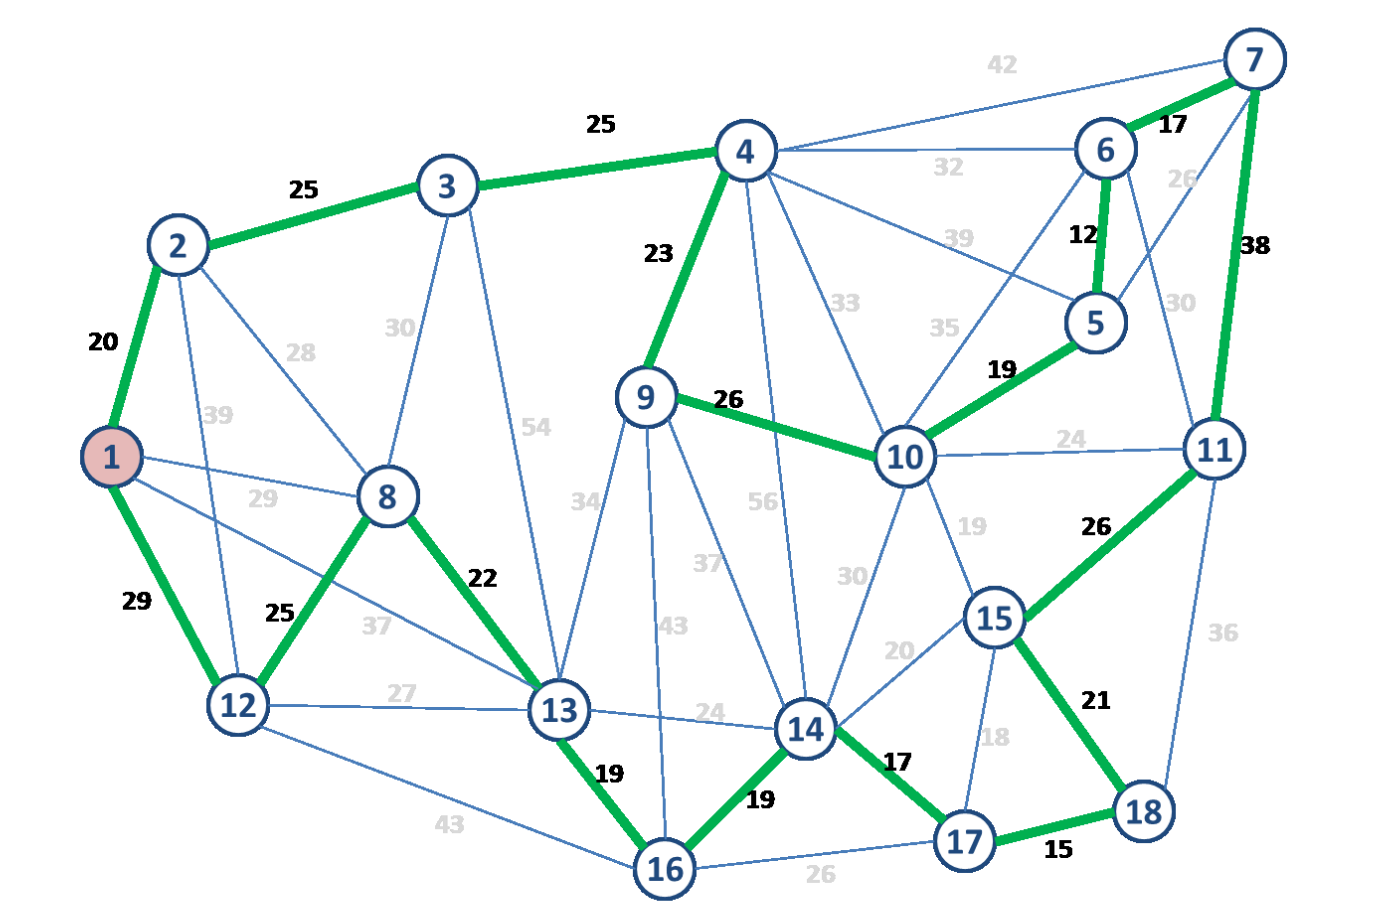
\includegraphics[scale=0.22]{img/tsp.png}
    \captionsetup{labelformat=empty}
    \caption{Exemplo com solução para o caixeiro viajante \cite{valeri2019}}
\end{figure}